\chapter{Estado del arte}

\section{Aplicaciones}

En el mercado, existen ya aplicaciones que cuentan con una temática parecida. Vamos a comentarlas a continuación.

\begin{itemize}

    \item \textbf{Handshake:} Es una aplicación disponible para dispositivos Android e iOS. Como podemos ver en la Figura~\ref{fig:handshake1} permite tomar decisiones en grupo sobre qué película o serie ver, dónde cenar, qué receta hacer, qué vino tomar, decidir el nombre de un bebé o crear tu elección personalizada. Para tomar decisiones se crea una sala con un código a la cual se pueden unir el resto de compañeros, tal como se ve en la Figura~\ref{fig:handshake2}. Entre sus carencias, encontramos que al elegir una película, no permite ver la descripción y se queda en un proceso de elección infinito que es necesario parar manualmente. Asimismo, dispone de anuncios y algunas opciones de pago, como puede observarse en la Figura~\ref{fig:handshake3}.

    \begin{figure}[ht]
        \centering
        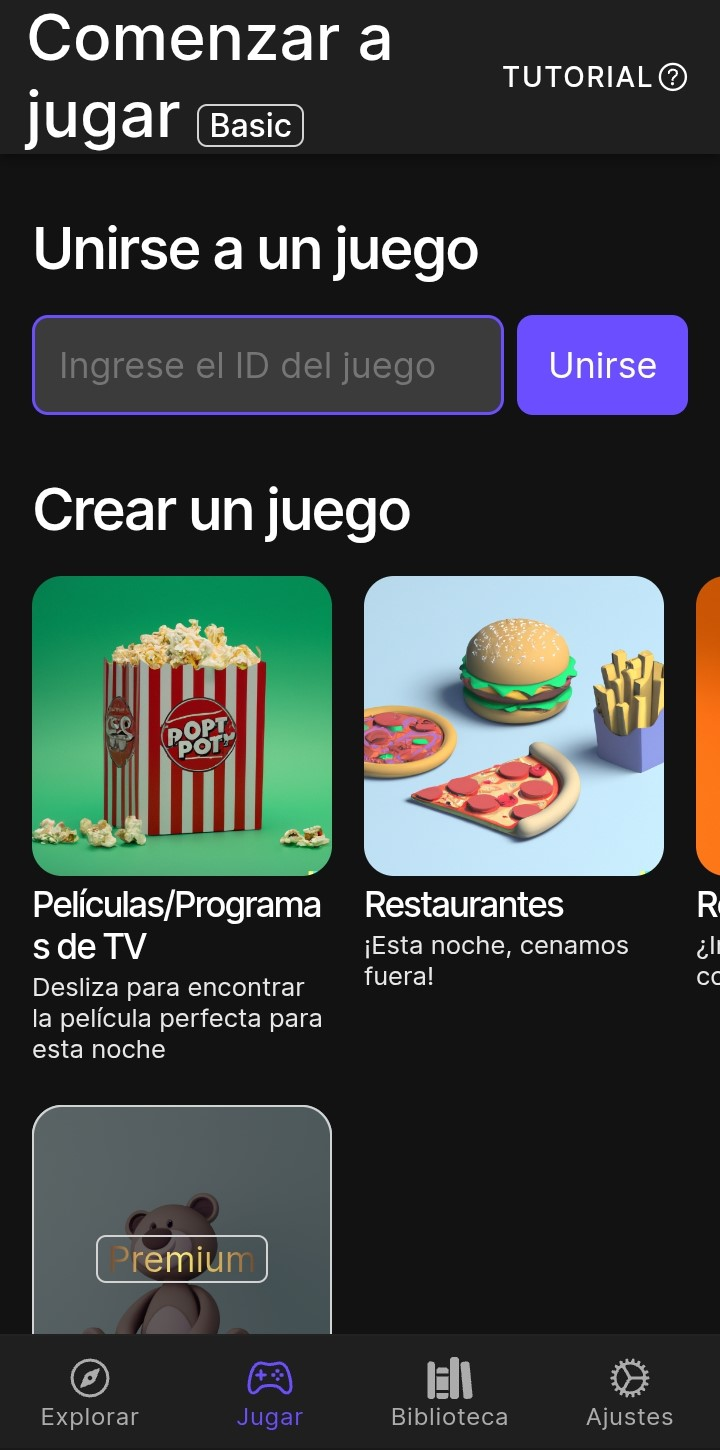
\includegraphics[width=\tamApps\textwidth]{figuras/estado_arte/apps/Handshake1.jpeg}
        \caption{Handshake página principal}
        \label{fig:handshake1}
    \end{figure}

    \begin{figure}[ht]
        \centering
        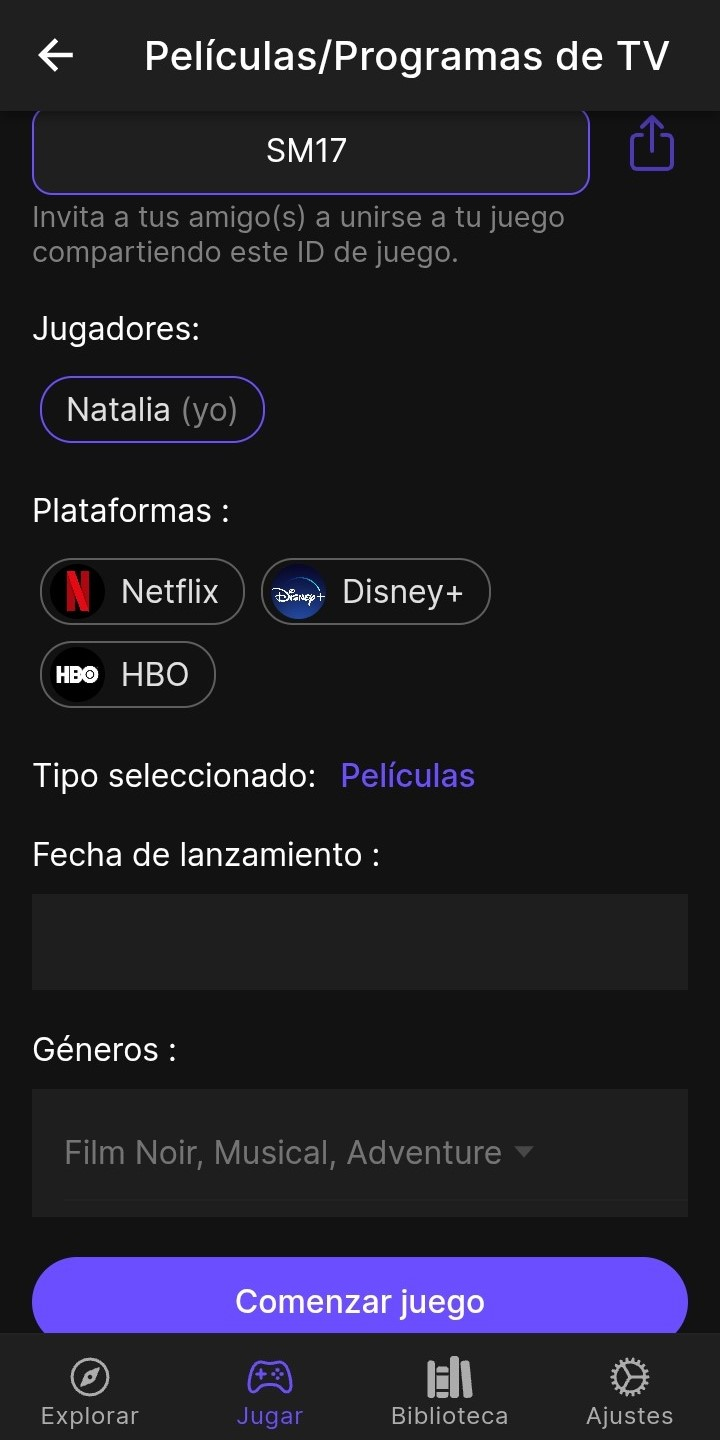
\includegraphics[width=\tamApps\textwidth]{figuras/estado_arte/apps/Handshake2.jpeg}
        \caption{Handshake creación de una sala}
        \label{fig:handshake2}
    \end{figure}

    \begin{figure}[ht]
        \centering
        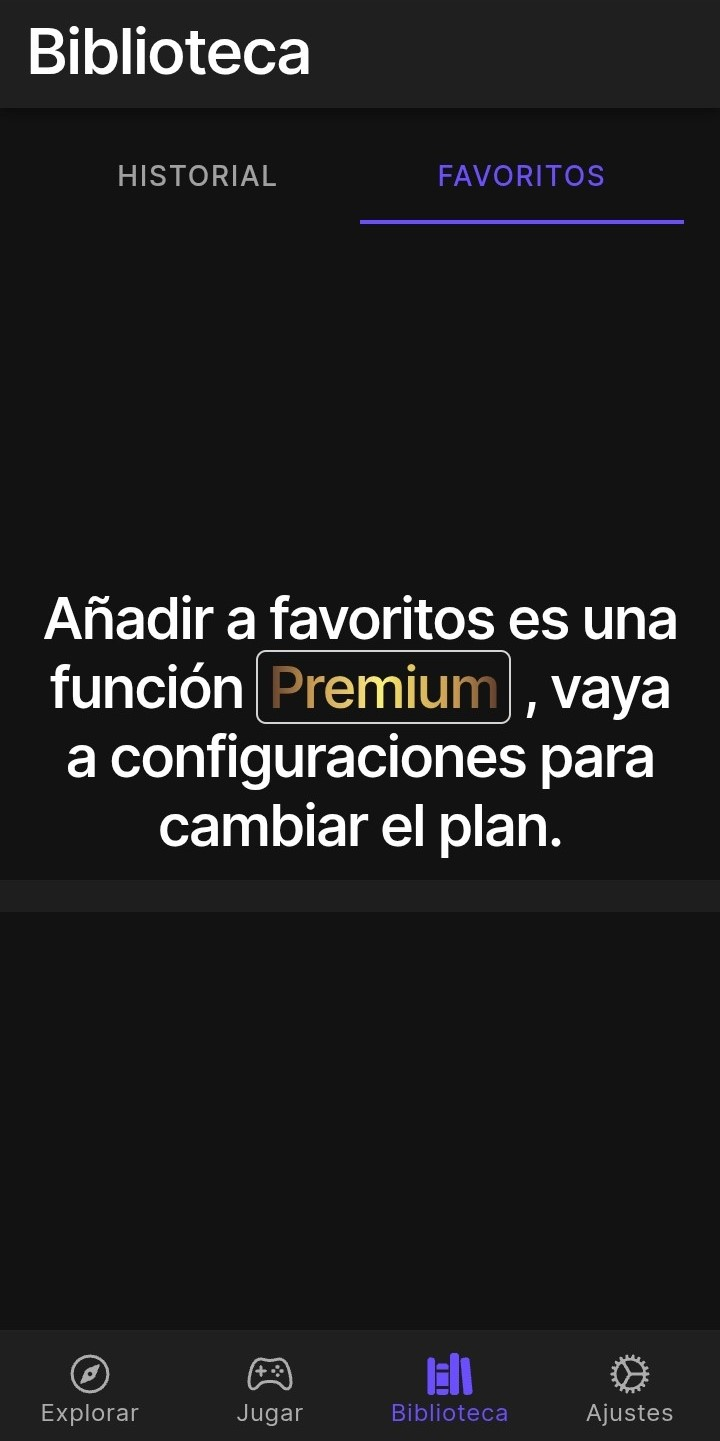
\includegraphics[width=\tamApps\textwidth]{figuras/estado_arte/apps/Handshake3.jpeg}
        \caption{Handshake opción premium}
        \label{fig:handshake3}
    \end{figure}
    
    \item \textbf{\href{https://feverup.com/es}{Fever} \cite{fever2026home}:}  Está disponible en Android e iOS. Según se ilustra en la Figura~\ref{fig:Fever1}  recomienda de manera individual distintas actividades culturales con coste en una ciudad. Permite elegir entre un listado o en un mapa.

    \begin{figure}[ht]
        \centering
        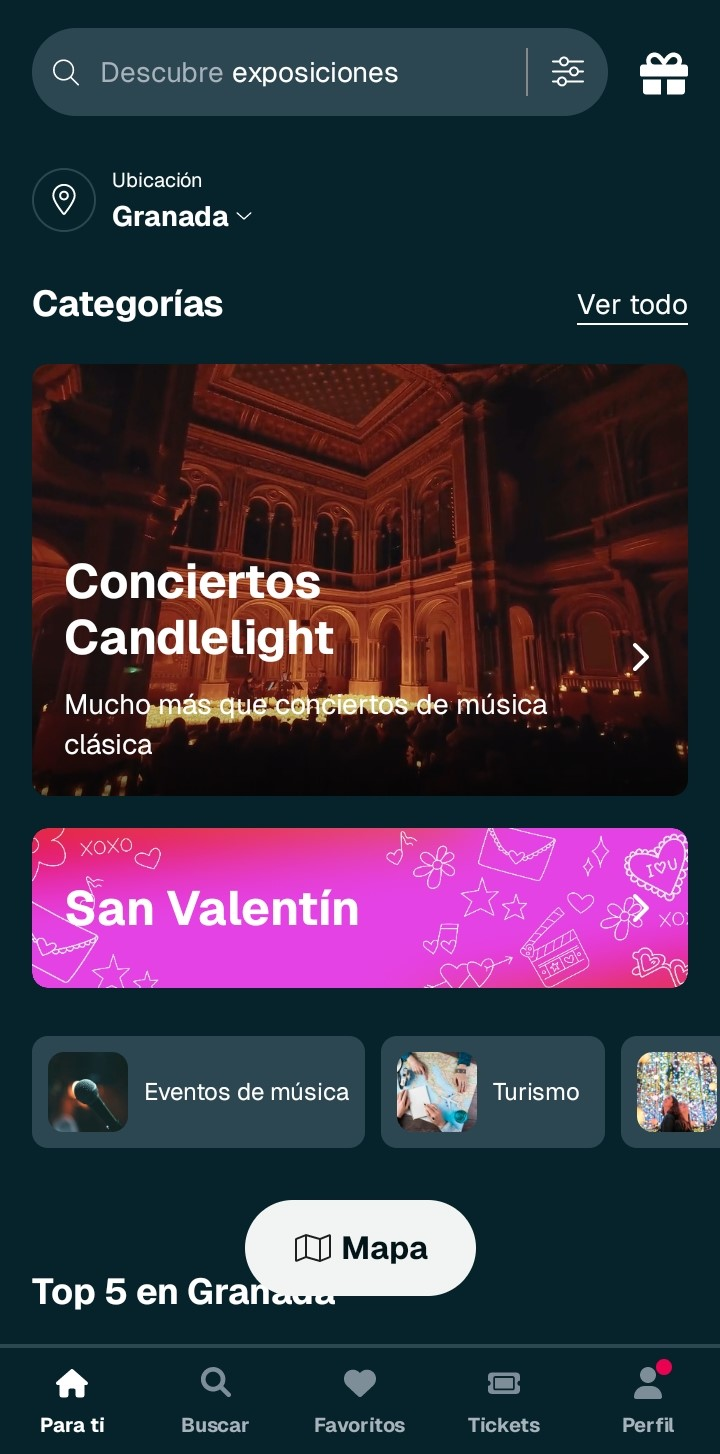
\includegraphics[width=\tamApps\textwidth]{figuras/estado_arte/apps/Fever1.jpeg}
        \caption{Fever página principal}
        \label{fig:Fever1}
    \end{figure}
    
    \item \textbf{\href{https://www.thefork.es/}{TheFork} \cite{thefork2026home}:} Funciona tanto en Android como en iOS. Su funcionamiento es encontrar restaurantes en tu ciudad, pudiendo visualizarlos en un mapa o un listado, tal como vemos en la Figura~\ref{fig:thefork1}. Además, permite añadir ejemplos a la busqueda y reservar en el que finalmente decidas.

    \begin{figure}[ht]
        \centering
        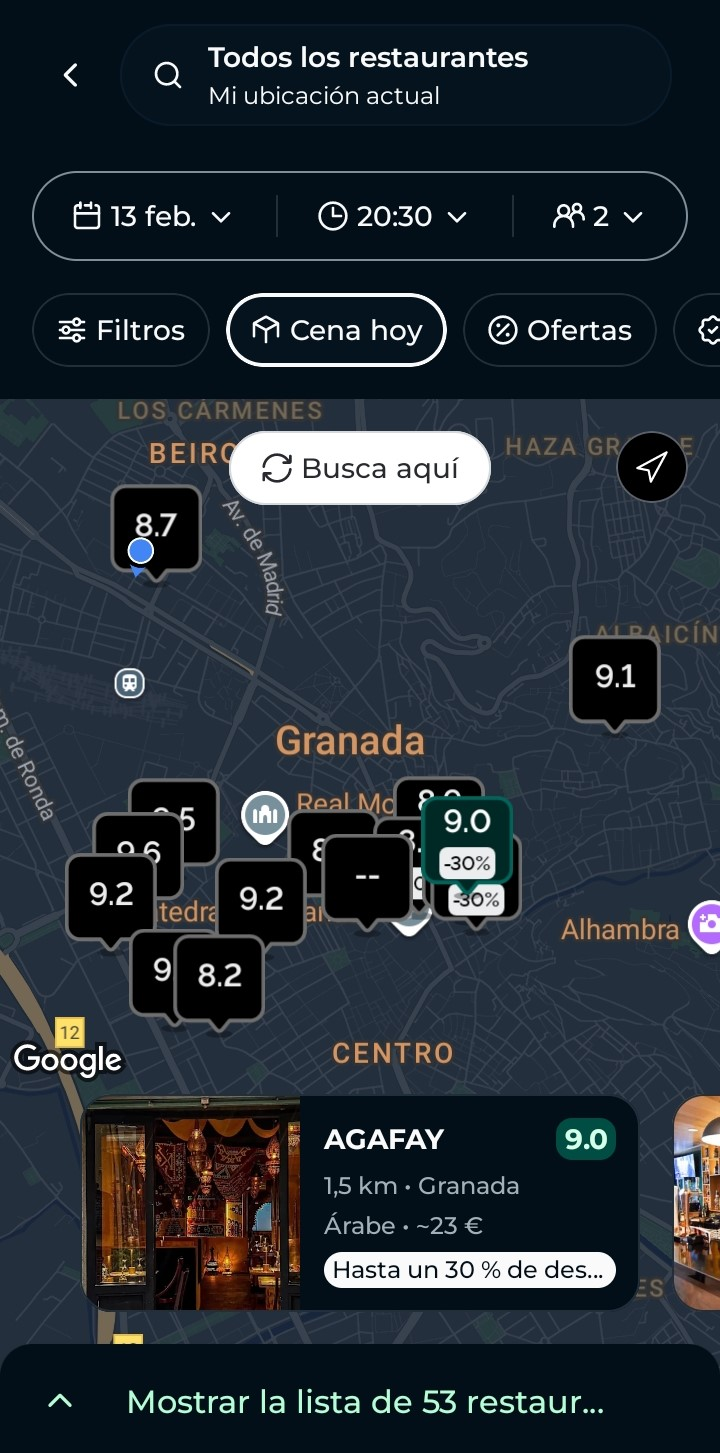
\includegraphics[width=\tamApps\textwidth]{figuras/estado_arte/apps/TheFork1.jpeg}
        \caption{TheFork resultado de una busqueda}
        \label{fig:thefork1}
    \end{figure}
    
    \item \textbf{\href{https://www.2nite.app/}{2NITE} \cite{2nite2026home}:} Se trata de una solución multiplataforma con soporte nativo para los sistemas operativos iOS y Android. Aporta informción sobre eventos musicales en localizaciones diversas como conciertos, bares, clubs, etc. Como podemos apreciar en la Figura~\ref{fig:2nite1} permite filtrar la información con diversos filtros tales como por ciudad o género musical. Asimismo, facilita información exclusiva de preventa, da recomendaciones personalizadas y permite comparar el precio de distintos proveedores de entradas como se muestra en la Figura~\ref{fig:2nite2}.

    \begin{figure}[ht]
        \centering
        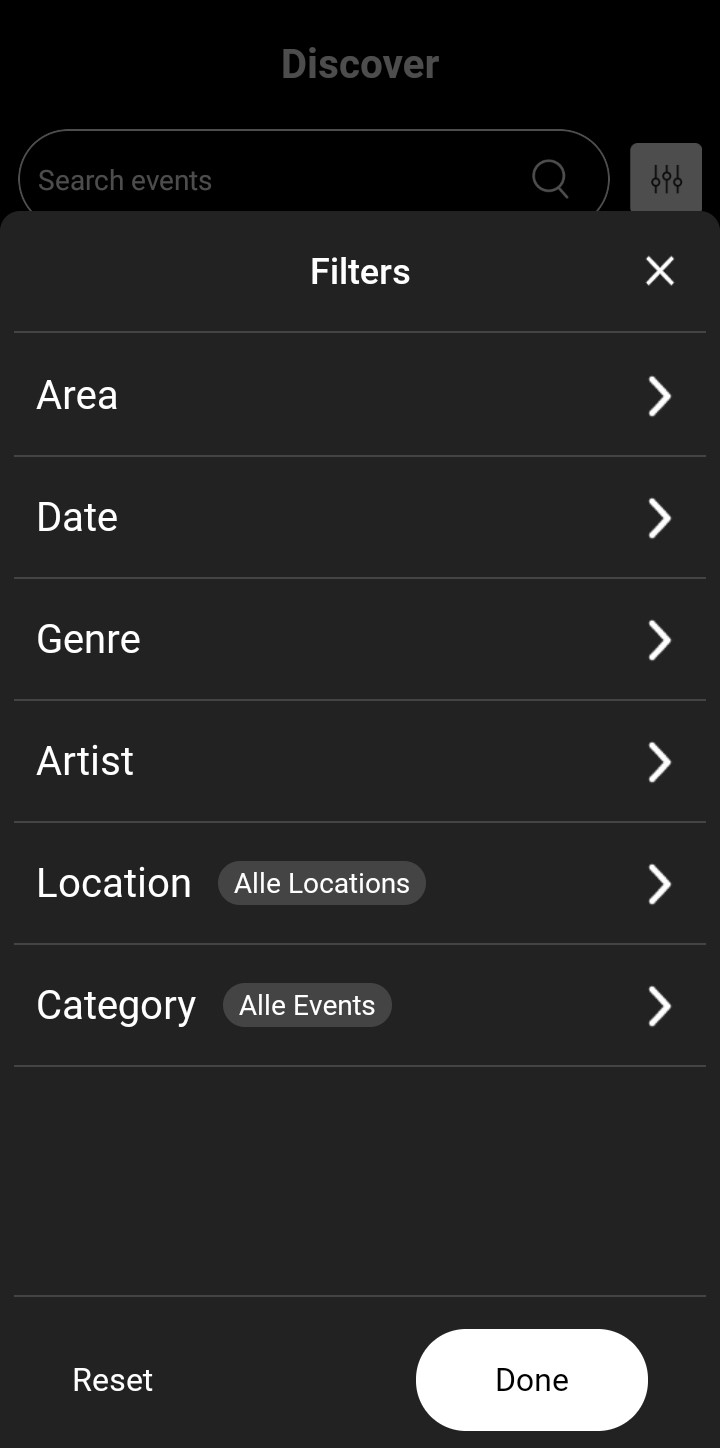
\includegraphics[width=\tamApps\textwidth]{figuras/estado_arte/apps/2NITE1.jpeg}
        \caption{2NITE opciones de filtrado}
        \label{fig:2nite1}
    \end{figure}

    \begin{figure}[ht]
        \centering
        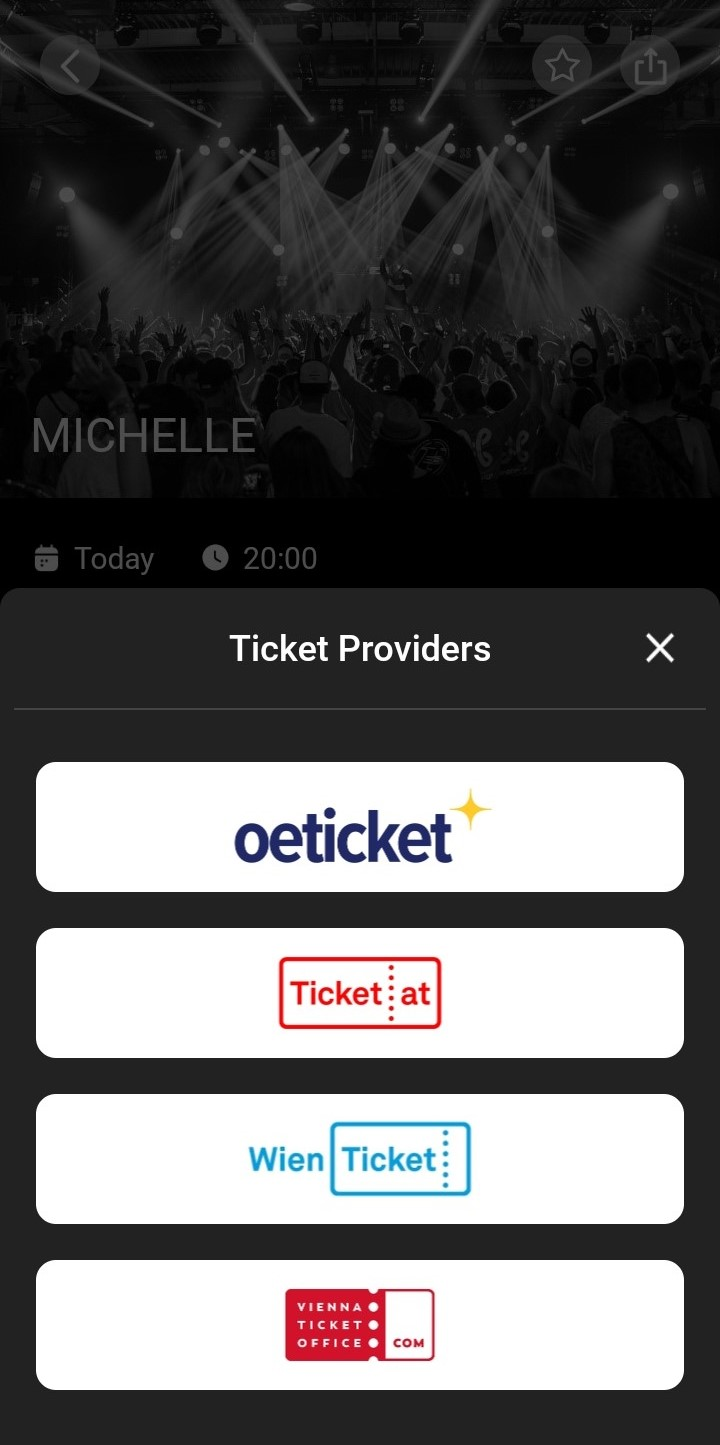
\includegraphics[width=\tamApps\textwidth]{figuras/estado_arte/apps/2NITE2.jpeg}
        \caption{2NITE opciones de compra de entradas}
        \label{fig:2nite2}
    \end{figure}


    \item \textbf{\href{https://daccordapp.com/}{Daccord} \cite{daccord2026home}:} Es una herramienta desarrollada para su ejecución en dispositivos móviles con arquitectura Android. Su función es permitir tomar decisiones en grupo, pudiendo crear o unirte a una sala mediante un código de tres palabras. Permite elegir tu nombre de usuario y foto de perfil eligiendo entre unos iconos que tienen de modelo. Además, de poder ponerlo en modo claro u oscuro. En este momento, solo permite crear una lista de opciones con descripción y opcionalmente incluirle una foto a cada una de ellas. No obstante, tanto insertar una imagen como crear un grupo de decisión generan una excepción como podemos observar en la Figura~\ref{fig:daccord1}. Al tratarse de una herramienta reciente, diversas funcionalidades se encuentran aún en fase de desarrollo como ilustra la Figura~\ref{fig:daccord2}, tales como temáticas predefinidas (películas, restaurantes, juegos, deportes y viajes) y utilidades como botones para poner un tiempo límite para decidir o permitir elegir una opción como no negocible. En estos momentos, solo está disponible en inglés.

    \begin{figure}[ht]
        \centering
        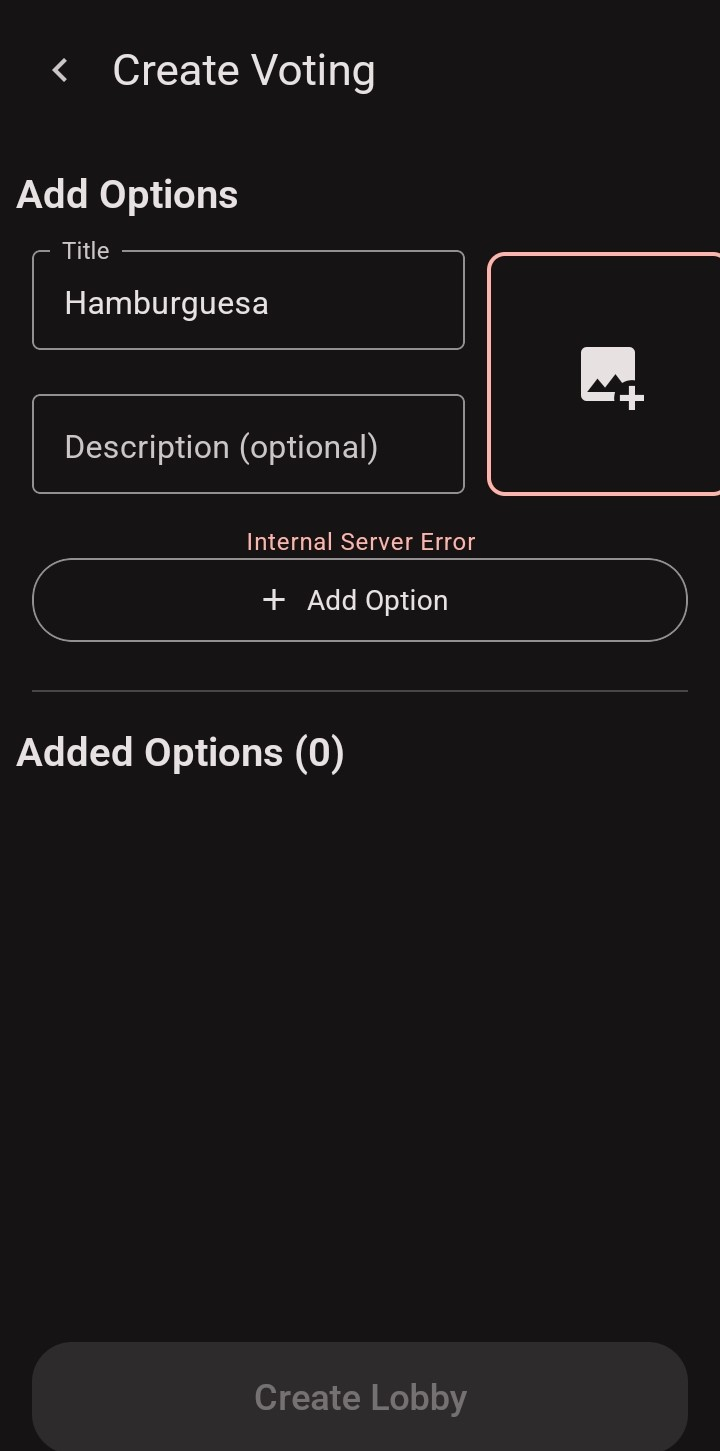
\includegraphics[width=\tamApps\textwidth]{figuras/estado_arte/apps/Daccord1.jpeg}
        \caption{Daccord error al insertar una imagen}
        \label{fig:daccord1}
    \end{figure}

    \begin{figure}[ht]
        \centering
        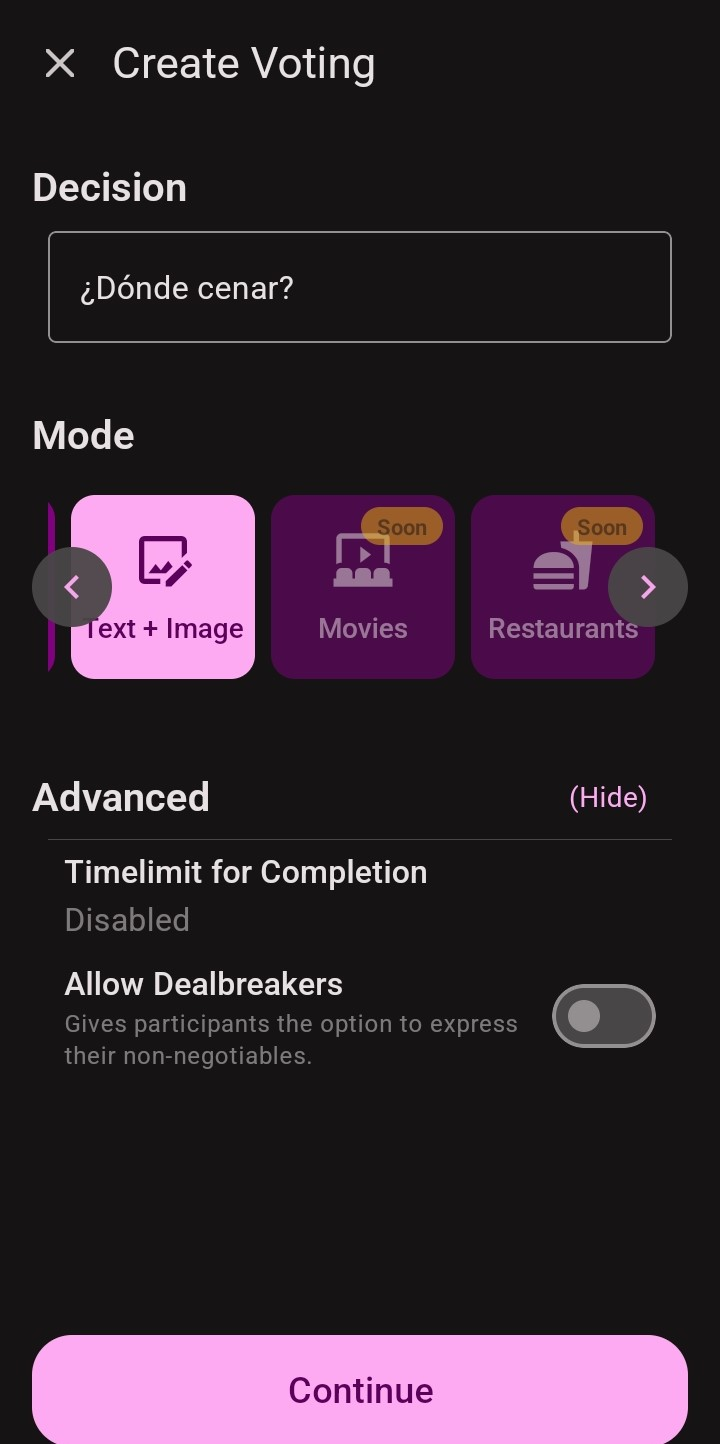
\includegraphics[width=\tamApps\textwidth]{figuras/estado_arte/apps/Daccord2.jpeg}
        \caption{Daccord temáticas en desarrollo}
        \label{fig:daccord2}
    \end{figure}
    

    \item \textbf{\href{https://tinydecisions.app/}{Tiny Decisions} \cite{tinydecisions2026home}:} La plataforma se encuentra accesible para usuarios tanto de terminales Android como iPhone. Su función es de toma de decisiones individuales o en grupo desde un mismo dispositivo pudiendo elegirse tal como podemos ver en la Figura~\ref{fig:tinydecisions1} mediante una ruleta, poner un dedo por persona en la pantalla y seleccionar aleatoriamente uno, sacar un número o lanzar una moneda. Como se observa en la Figura~\ref{fig:tinydecisions2} tiene muchas opciones de ruletas por defecto y permite crear las tuyas propias pudiendo personalizar el color de las opciones y organizar las ruletas por etiquetas. Asimismo, dispone de modo claro y osucuro y está traducida en distintos idiomas. Adicionalmente, tiene disponible opciones premium como eliminar los anuncios, ponerle distinto peso a las opciones de la ruleta, elegir más de un dedo, etc.

    \begin{figure}[ht]
        \centering
        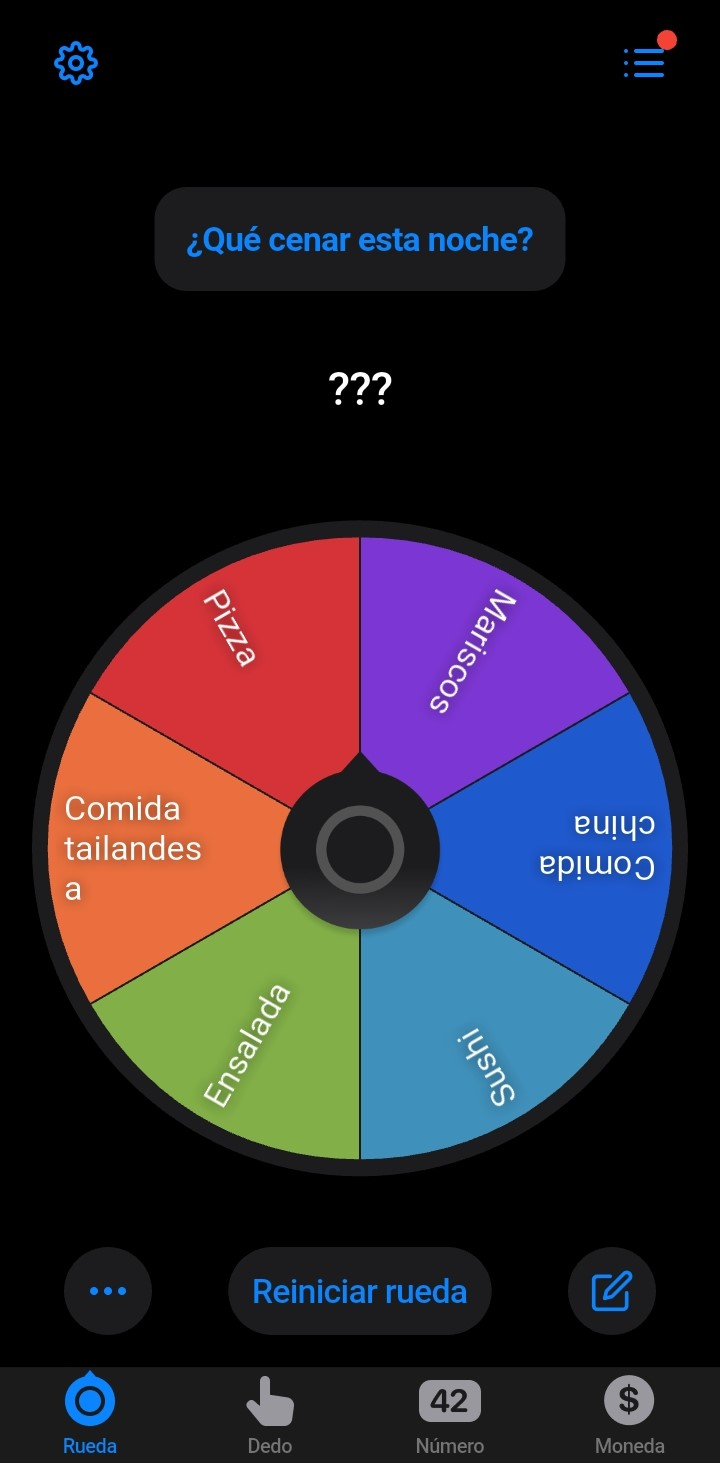
\includegraphics[width=\tamApps\textwidth]{figuras/estado_arte/apps/TinyDecisions1.jpeg}
        \caption{TinyDecisions página principal}
        \label{fig:tinydecisions1}
    \end{figure}

    \begin{figure}[ht]
        \centering
        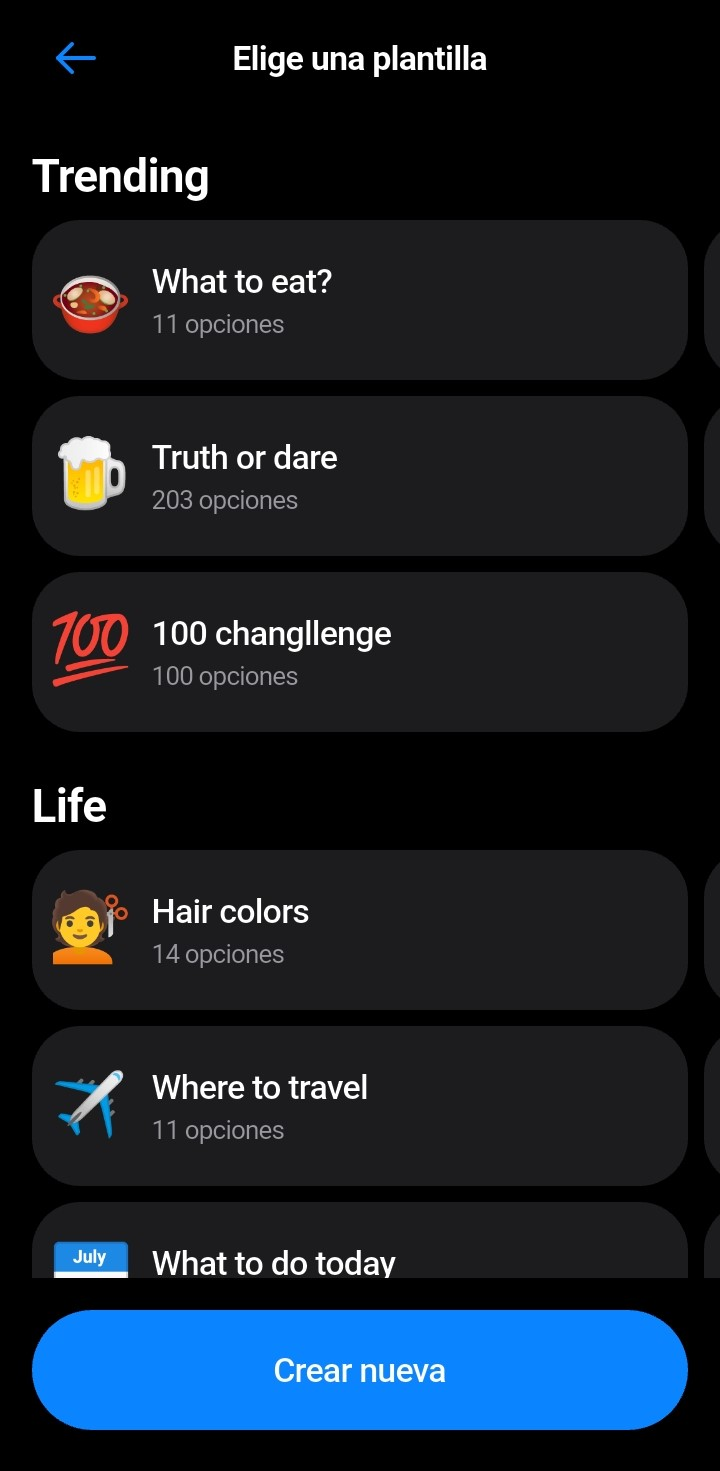
\includegraphics[width=\tamApps\textwidth]{figuras/estado_arte/apps/TinyDecisions2.jpeg}
        \caption{TinyDecisions ruletas por defecto}
        \label{fig:tinydecisions2}
    \end{figure}
    
    \item \textbf{ChoicePro:} Es una herramienta desarrollada para dispositivos Android. Permite tomar decisiones de manera individualizada mediante una ruleta o de manera científica. En la segunda modalidad, el usuario puntua las distintas alternativas mediante unos criterios personalizados y una prioridad ajustable, aportando al final las puntuaciones de las distintas opciones e indicándo la óptima, como se puede apreciar en la Figura~\ref{fig:choicepro1}.

    \begin{figure}[ht]
        \centering
        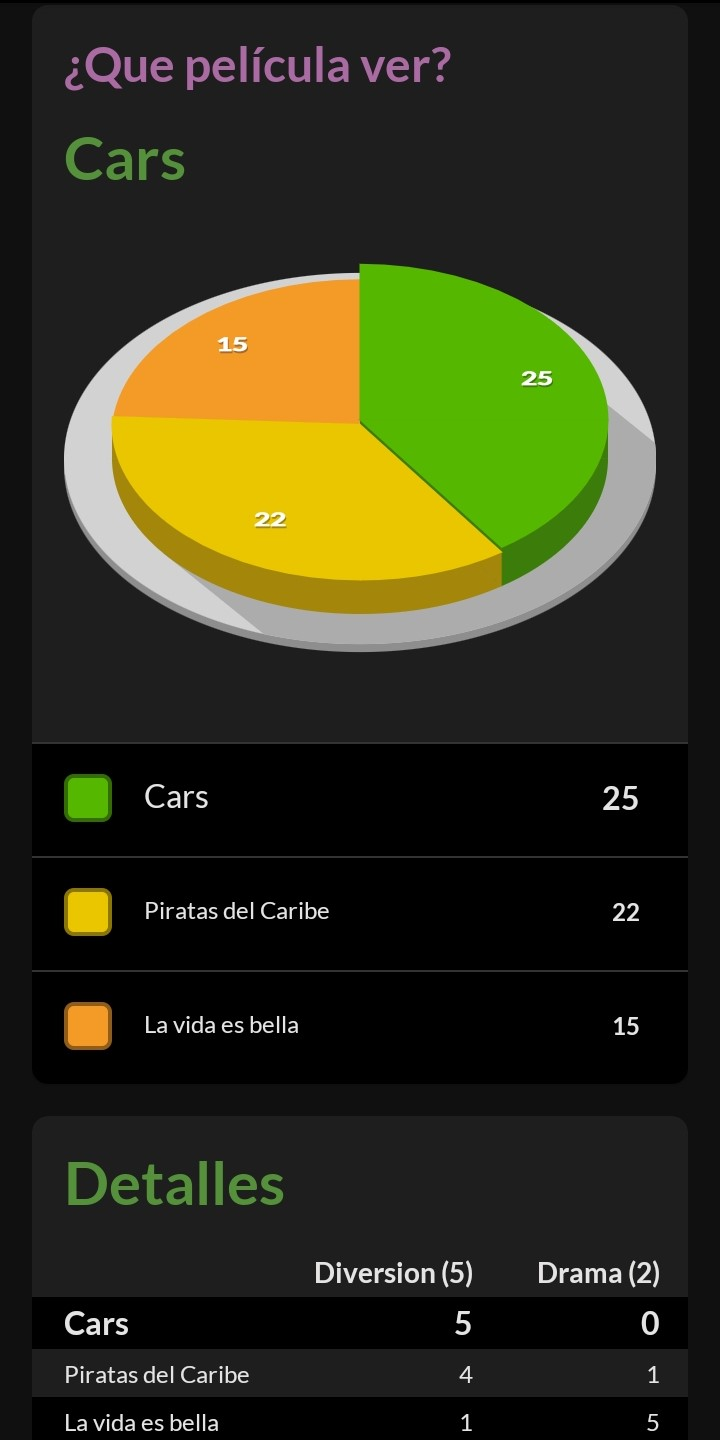
\includegraphics[width=\tamApps\textwidth]{figuras/estado_arte/apps/ChoicePro1.jpeg}
        \caption{ChoicePro resultado de manera científica}
        \label{fig:choicepro1}
    \end{figure}

    \item \textbf{Rank it!:} Es una aplicación disponible para Android. Ayuda a la toma de decisiones de manera individual o en grupo desde un mismo dispositivo. Permite que haya hasta doce opciones y hasta diez jugadores. La decisión como podemos observar en la Figura~\ref{fig:rankit1} se toma de manera aleatoria con una ruleta o mediante un ranking que hacen los jugadores por turnos. Si la decisión final es un empate tal como muestra la Figura~\ref{fig:rankit2}, se elije entre las opciones empatadas de manera aleatoria o elije el dueño del dispositivo. Al hacer una nueva partida permite conservar las opciones y/o los jugadores. 

    \begin{figure}[ht]
        \centering
        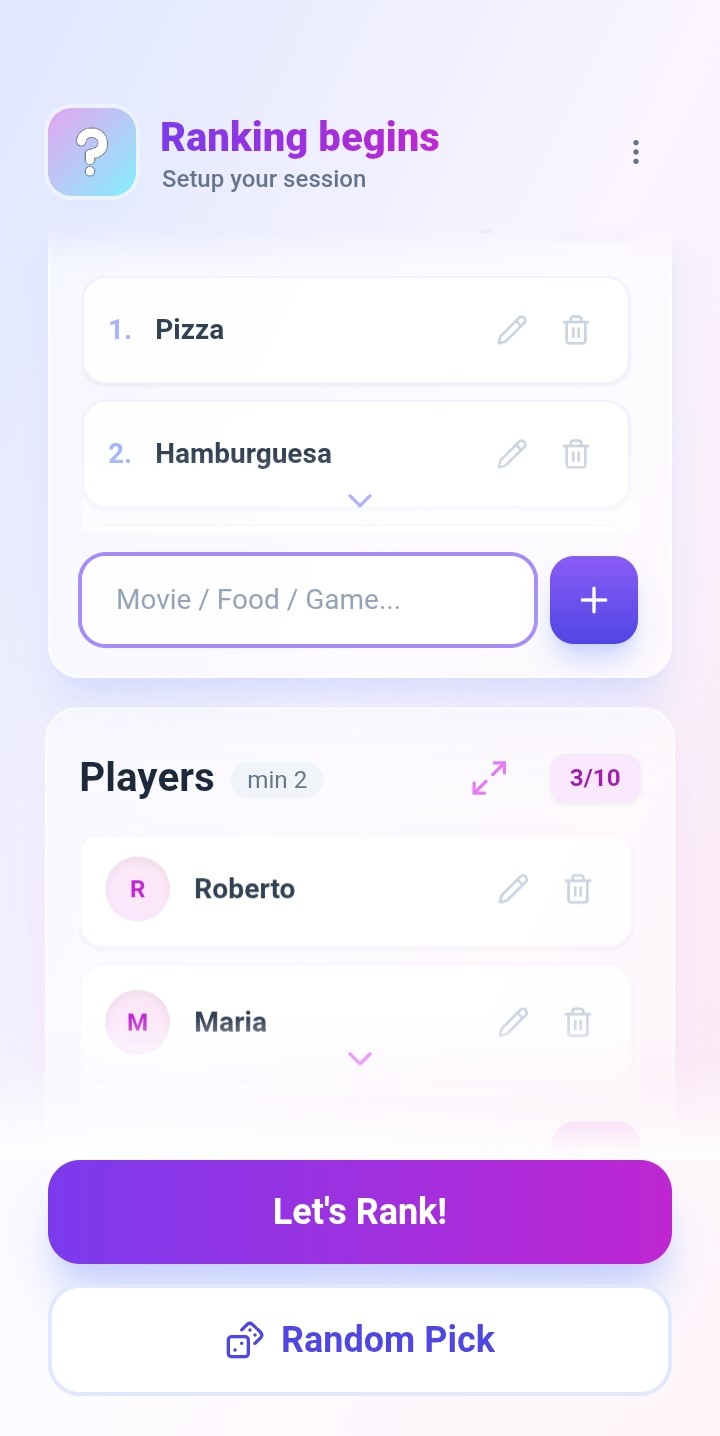
\includegraphics[width=\tamApps\textwidth]{figuras/estado_arte/apps/Rankit1.jpeg}
        \caption{Rank it! página principal}
        \label{fig:rankit1}
    \end{figure}

    \begin{figure}[ht]
        \centering
        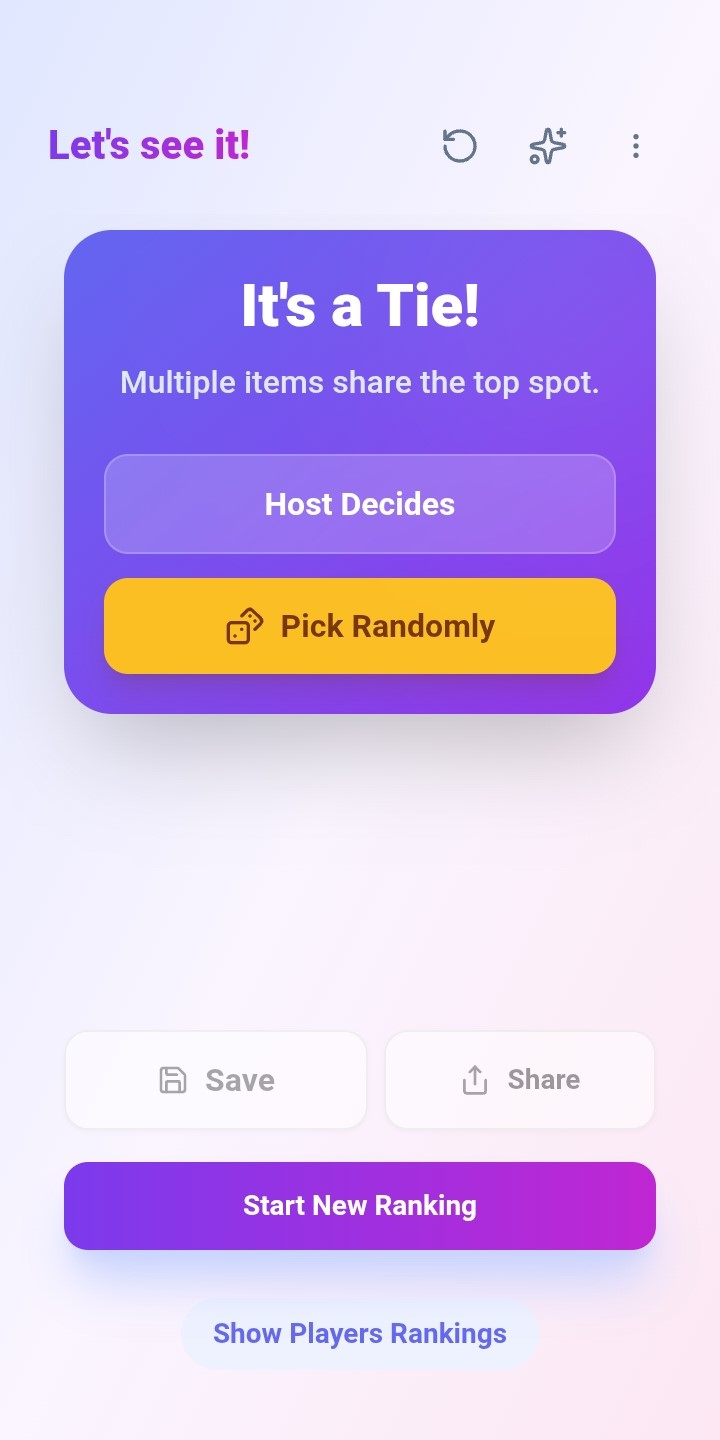
\includegraphics[width=\tamApps\textwidth]{figuras/estado_arte/apps/Rankit2.jpeg}
        \caption{Rank it! empate}
        \label{fig:rankit2}
    \end{figure}
    
\end{itemize}














\section{Posibles tecnologías a usar}

\subsection{Front-End} 

Algunas de las posibles tecnologías front-end que más se alinean con los objetivos de esta aplicación son \cite{redwerk2024herramientas}: 


\begin{itemize}

    \item \textbf{\href{https://flutter.dev/}{Flutter} \cite{flutter2026home} (\ref{fig:flutterlogo}):} Framework de Google que permite el desarrollo multiplataforma en iOS, Android, Web y Desktop con un único código fuente. Usa su propio motor gráfico, lo que le proporciona un buen rendimiento y una interfaz consistente. Tiene un desarrollo rápido y permite crear interfaces visuales complejas. Posee una amplia biblioteca de widgets y elementos de interfaz de usuario prediseñados.

    \begin{figure}[ht]
        \centering
        
\includegraphics[width=\tamApps\textwidth]{figuras/estado_arte/tecnologias/flutter_logo.png}
        \caption{Flutter Logo}
        \label{fig:flutterlogo}
    \end{figure}

    \item \textbf{\href{https://reactnative.dev/}{React Native} \cite{reactnative2026home}:} Framework basado en React que permite el desarrollo multiplataforma usando tecnologías web. El código se traduce a componentes nativos, logrando un rendimiento cercano al nativo. Consta de una gran comunidad, amplias bibliotecas y plugins de terceros. Sin embargo, algunas funcionalidades nativas pueden requerir módulos personalizados. Además, el rendimiento se puede ver afectado en tareas complejas.

    \begin{figure}[ht]
        \centering
        
\includegraphics[width=\tamApps\textwidth]{figuras/estado_arte/tecnologias/reactnative_logo.png}
        \caption{React Native Logo}
        \label{fig:reactnativelogo}
    \end{figure}

     \item \textbf{\href{https://developer.android.com/}{Android SDK} \cite{androidsdk2026}:} Proporciona las herramientas necesarias para el desarrollo nativo en Android. Aporta el máximo rendimiento y acceso completo al hardware del dispositivo. El uso de lenguajes como Kotlin permite usar librerias y APIs nativas mejorando el rendimiento. Para utilizarlo podemos usar android studio como se ve en la Figura ~\ref{fig:androidstudiointerfaz}

     \begin{figure}[ht]
        \centering
        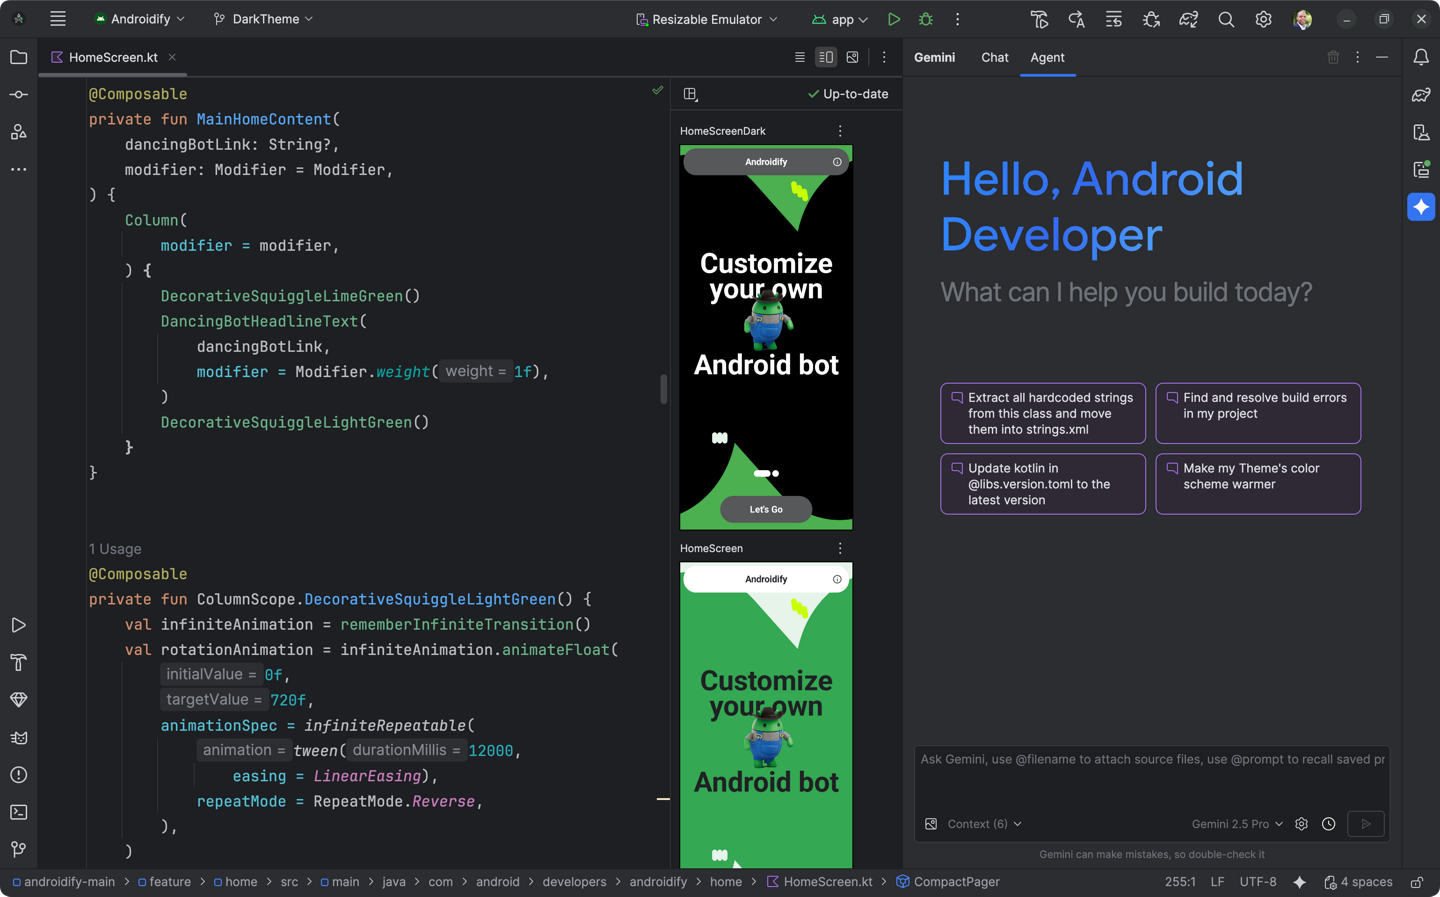
\includegraphics[width=\tamInterfaz\textwidth]{figuras/estado_arte/tecnologias/androidstudio.png}
        \caption{Android Studio Interfaz}
        \label{fig:androidstudiointerfaz}
    \end{figure}

      \item \textbf{\href{https://developer.apple.com/}{iOS SDK} \cite{iossdk2026}:} Tecnología oficial para el desarrollo nativo en iOS. Permite crear aplicaciones estables y altamente integradas, ofreciendo un alto rendimiento y un diseño acorde a Apple. Se puede programar con la interfaz que proporciona Xcode como podemos observar en la Figura ~\ref{fig:xcodeinterfaz}

       \begin{figure}[ht]
        \centering
        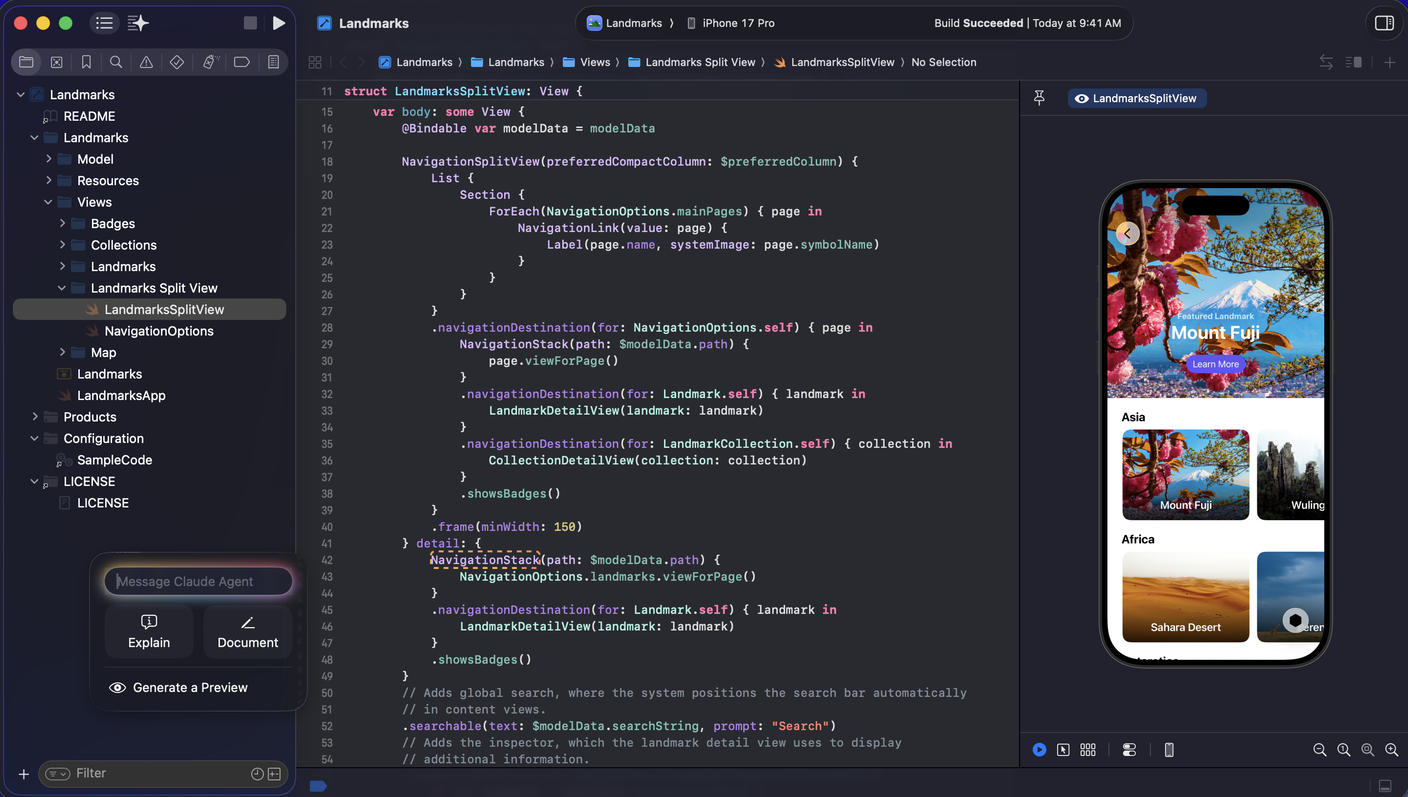
\includegraphics[width=\tamInterfaz\textwidth]{figuras/estado_arte/tecnologias/xcode_iOS.png}
        \caption{Xcode Interfaz}
        \label{fig:xcodeinterfaz}
    \end{figure}

      \item \textbf{\href{https://ionicframework.com/}{Ionic} \cite{ionic2026home} (\ref{fig:ioniclogo}):} Framework híbrido de desarrollo multiplataforma usando tecnologías web. Se ejecuta dentro de un contenedor web facilitando el desarrollo, pero reduciendo el rendimiento. Es adecuado para proyectos sencillos o prototipos.

      \begin{figure}[ht]
        \centering
        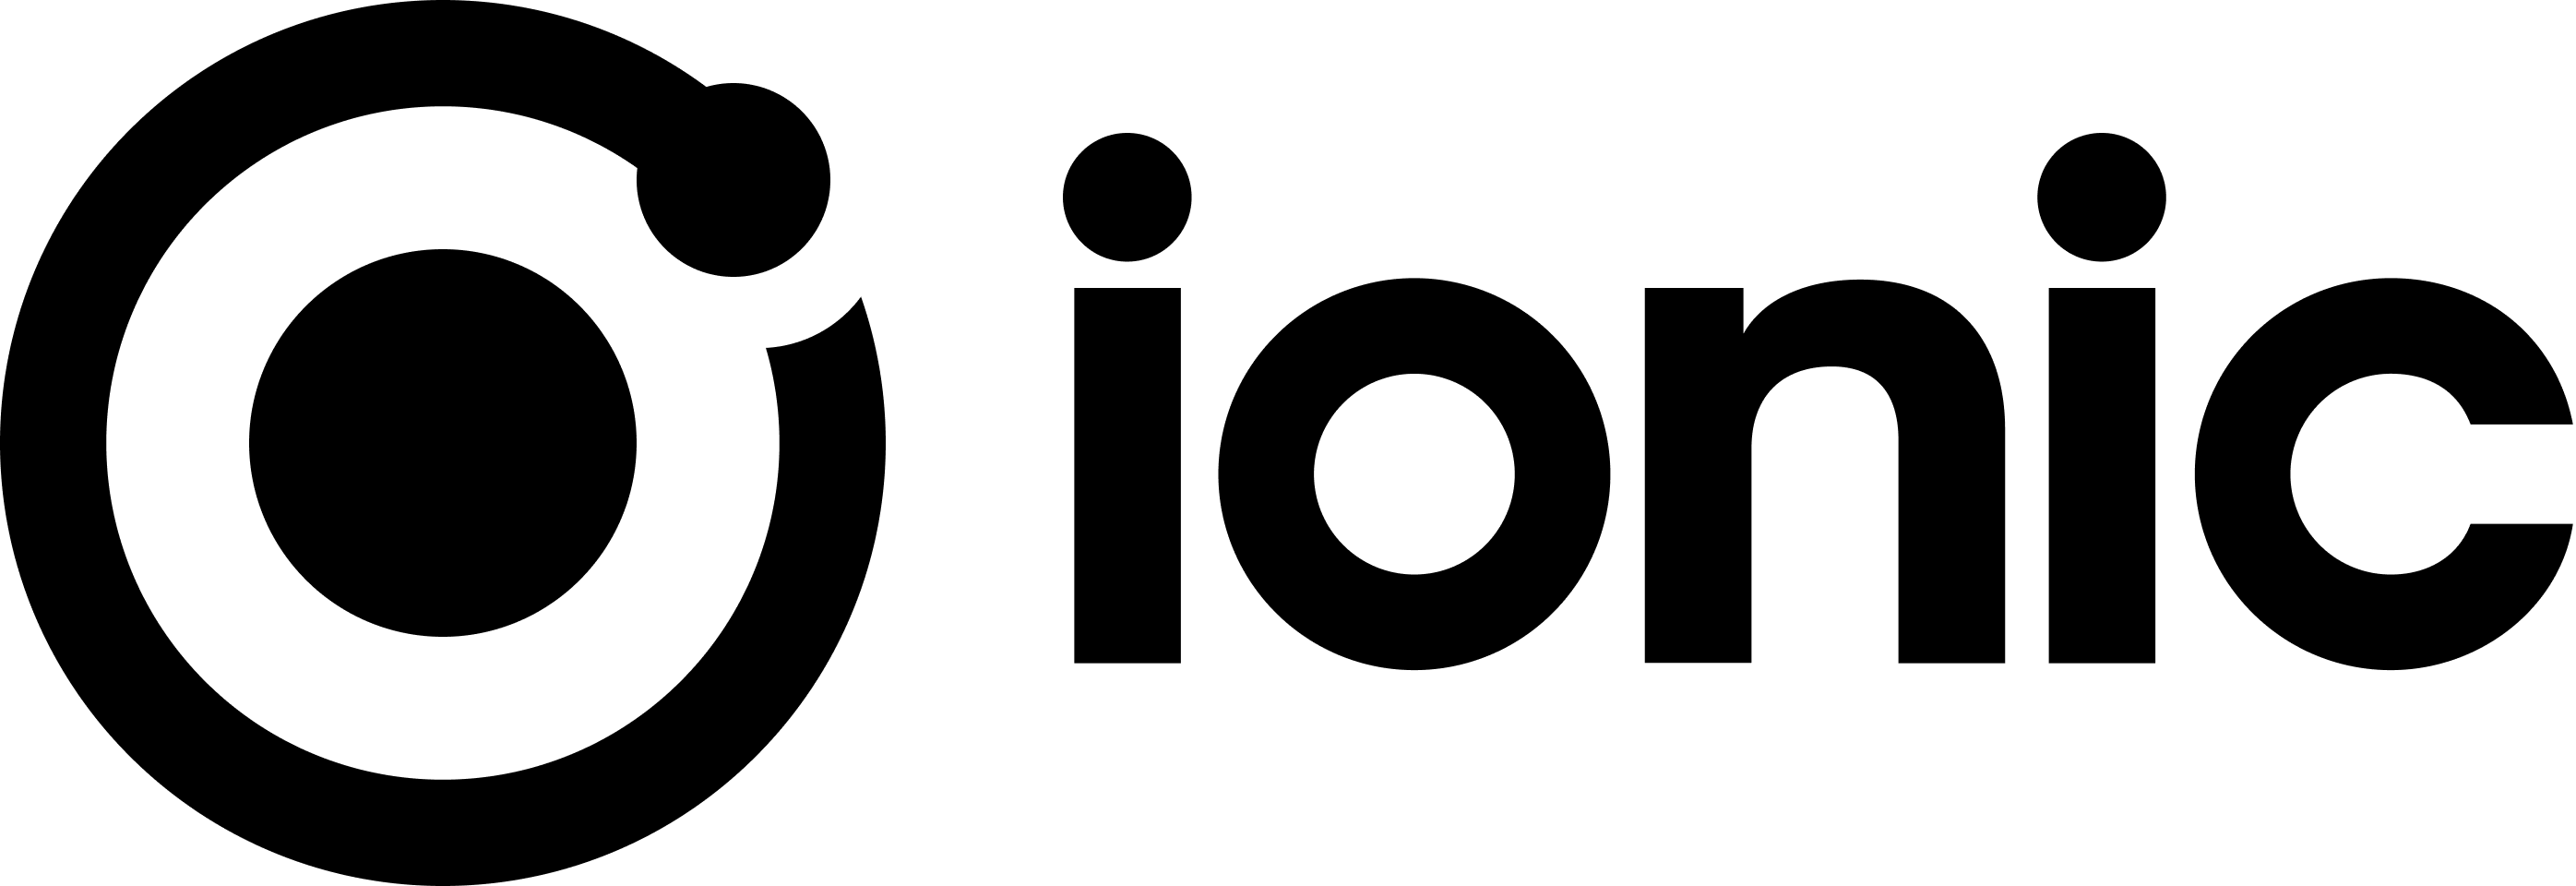
\includegraphics[width=\tamApps\textwidth]{figuras/estado_arte/tecnologias/ionic_logo.png}
        \caption{Ionic Logo}
        \label{fig:ioniclogo}
    \end{figure}

      \item \textbf{\href{https://dotnet.microsoft.com/es-es/apps/maui}{.NET MAUI} \cite{netmaui2026home} (\ref{fig:netmauilogo}): } Framework multiplataforma de Miccrosoft basado en el ecosistema .NET. Permite compartir gran parte del código entre Android e iOS, permitiendo acceder a funcionalidades nativas.

      \begin{figure}[ht]
        \centering
        
\includegraphics[width=\tamApps\textwidth]{figuras/estado_arte/tecnologias/net_logo.png}
        \caption{.NET MAUI Logo}
        \label{fig:netmauilogo}
    \end{figure}

      \item \textbf{\href{https://unity.com/es}{Unity} \cite{unity2026home}:} Motor de desarrollo multiplataforma que posee una gran interfaz gráfica y funciones de arrastre. Está escrito en C\# y posee un uso sencillo. Puede crear aplicaciones en 2D y 3D. Sin embargo, puede requerir plugins adicionales, ser excesivo para aplicaciones sencillas y tener un alto coste de licencias. Podemos usar su interfaz que presenta el aspecto que vemos en la Figura ~\ref{fig:Unityinterfaz}

      \begin{figure}[ht]
        \centering
        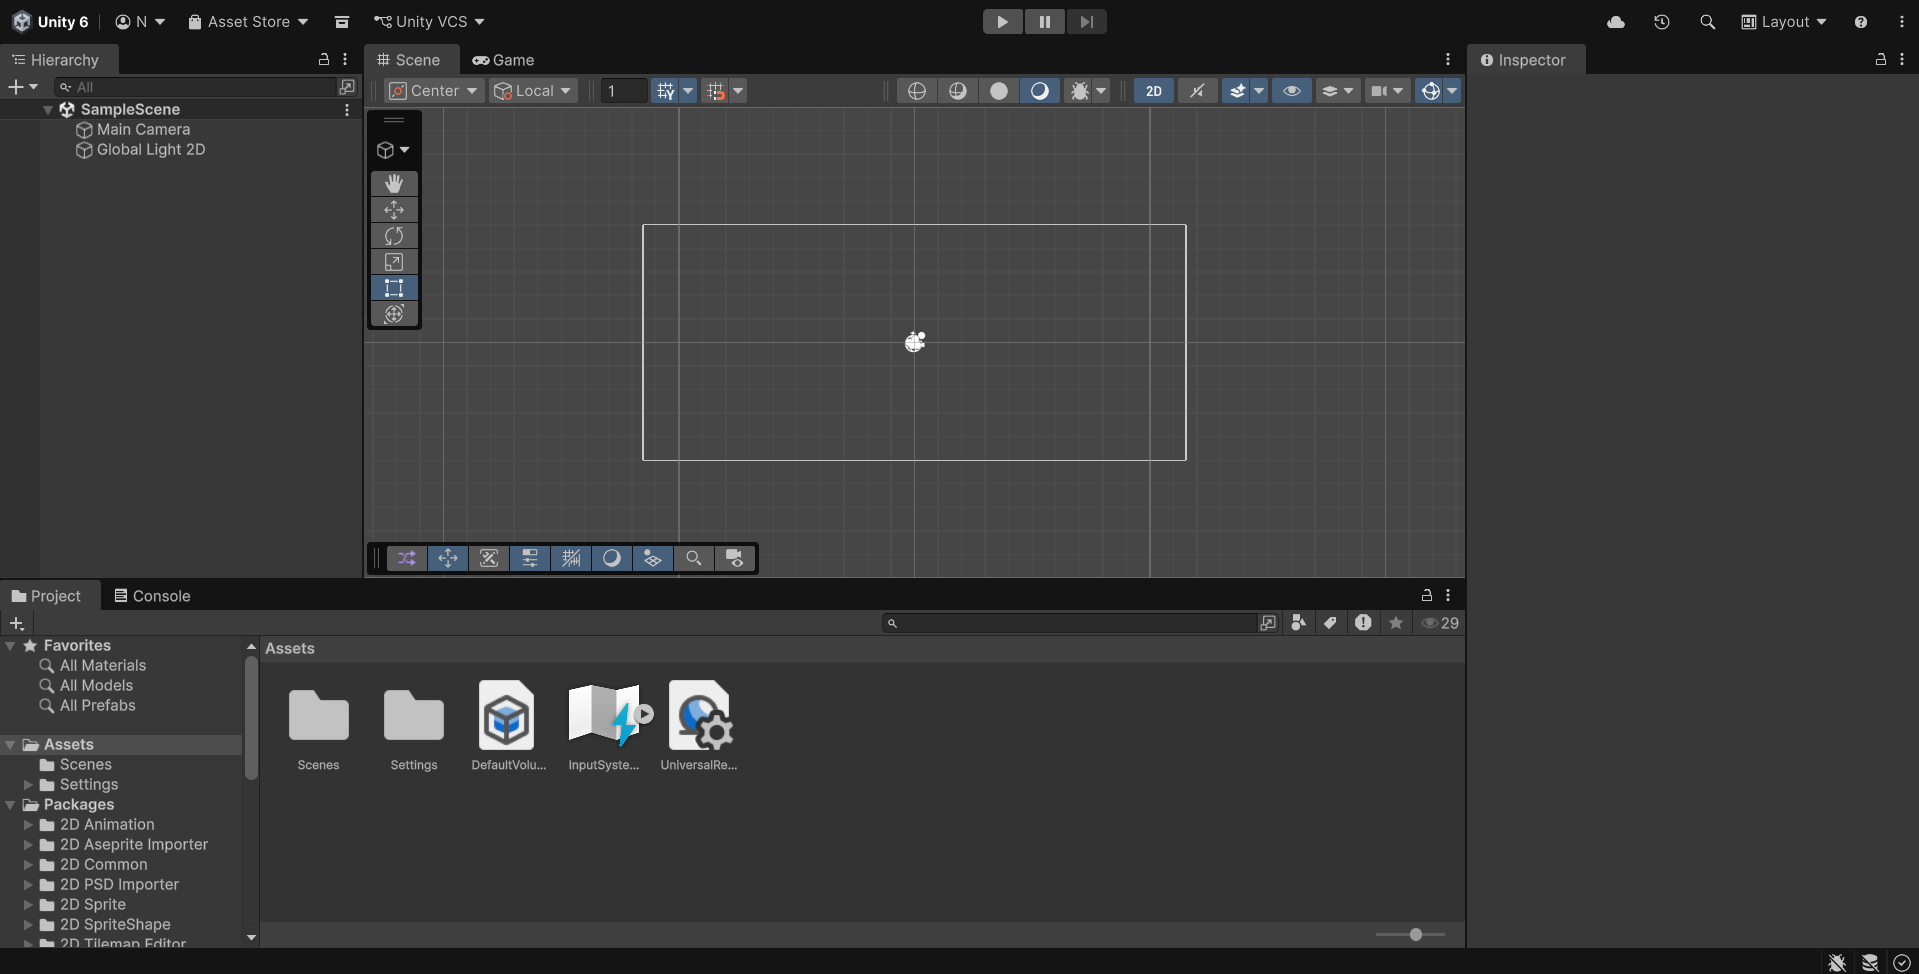
\includegraphics[width=\tamInterfaz\textwidth]{figuras/estado_arte/tecnologias/unityinterfaz.PNG}
        \caption{Unity Interfaz. Fuente: Elaboración propia}
        \label{fig:Unityinterfaz}
    \end{figure}

      \item \textbf{\href{https://nativescript.org/}{NativeScript} \cite{nativescript2026home} (\ref{fig:nativescriptlogo}):} Framework de desarrollo multiplataforma usando tecnologías web. Utiliza APIs y componentes nativos, dando un gran rendimiento. Posee un amplio conjunto de plugins, sin embargo la depuración puede ser compleja.

      \begin{figure}[ht]
        \centering
        
\includegraphics[width=\tamApps\textwidth * \real{0.65}]{figuras/estado_arte/tecnologias/nativescript-logo.png}
        \caption{NativeScript Logo}
        \label{fig:nativescriptlogo}
    \end{figure}

\end{itemize}
 
\subsection{Back-End}

\begin{itemize}

    \item \textbf{\href{https://www.djangoproject.com/}{Django} \cite{django2026home}:} Marco de desarrollo de Python ideal para aplicaciones grandes, CMS y proyectos que tienen que salir a producción rápidamente integrando seguridad. Incluye un panel de administración automático y un mapeo objeto-relacional para base de datos. Sin embargo, puede resultar pesado y tiene una estructura muy rígida. Como podemos apreciar en la Figura~\ref{fig:djangointerfaz} cuenta con un panel de administración propio.

     \begin{figure}[ht]
        \centering
        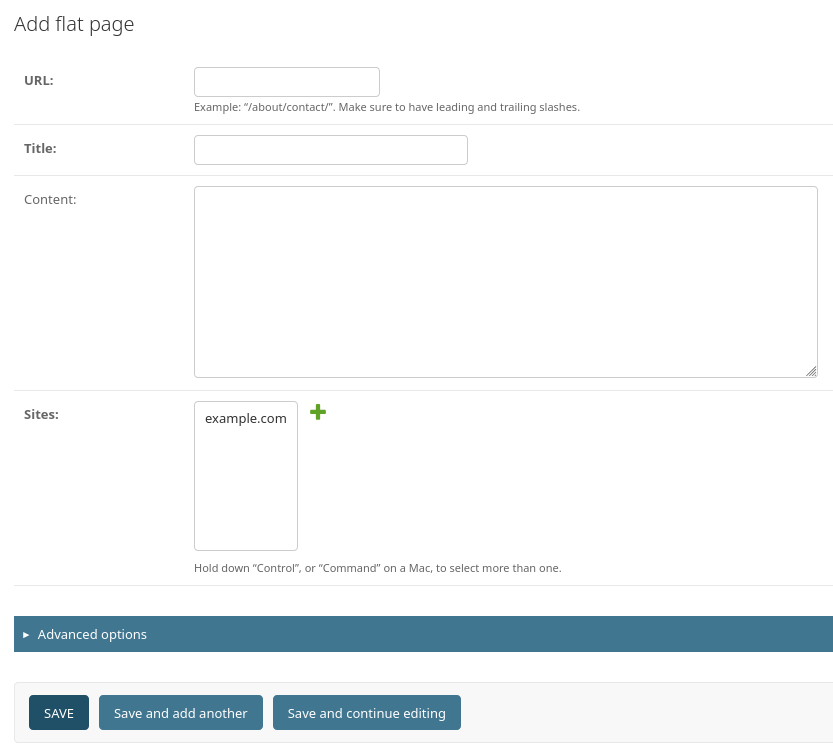
\includegraphics[width=\tamInterfaz\textwidth]{figuras/estado_arte/tecnologias/djangointerfaz.png}
        \caption{Django interfaz}
        \label{fig:djangointerfaz}
    \end{figure}
    
    \item \textbf{\href{https://flask.palletsprojects.com/en/stable/}{Flask} \cite{flask2026home} (\ref{fig:flasklogo}):} Microframework  del lenguaje Python enfocado en la simplicidad. Es usado en proyectos pequeños, prototipos rápidos y para tener control de cada componente. Destaca por ser muy ligero, flexible y de rápido aprendizaje.

    \begin{figure}[ht]
        \centering
        
\includegraphics[width=\tamApps\textwidth]{figuras/estado_arte/tecnologias/flasklogo.png}
        \caption{Flask Logo}
        \label{fig:flasklogo}
    \end{figure}

    \item \textbf{\href{https://fastapi.tiangolo.com/}{FastAPI} \cite{fastapi2026home}:} Plataforma de Python increíblemente rápido. Es muy utilizado para crear APIs de alto rendimiento, aplicacioens de Machine Learning y sistemas asíncronos. Además, genera documentación interactiva automáticamente. Cuenta con la interfaz Swagger que podemos visualizar en la Figura ~\ref{fig:swaggerinterfaz}

    \begin{figure}[ht]
        \centering
        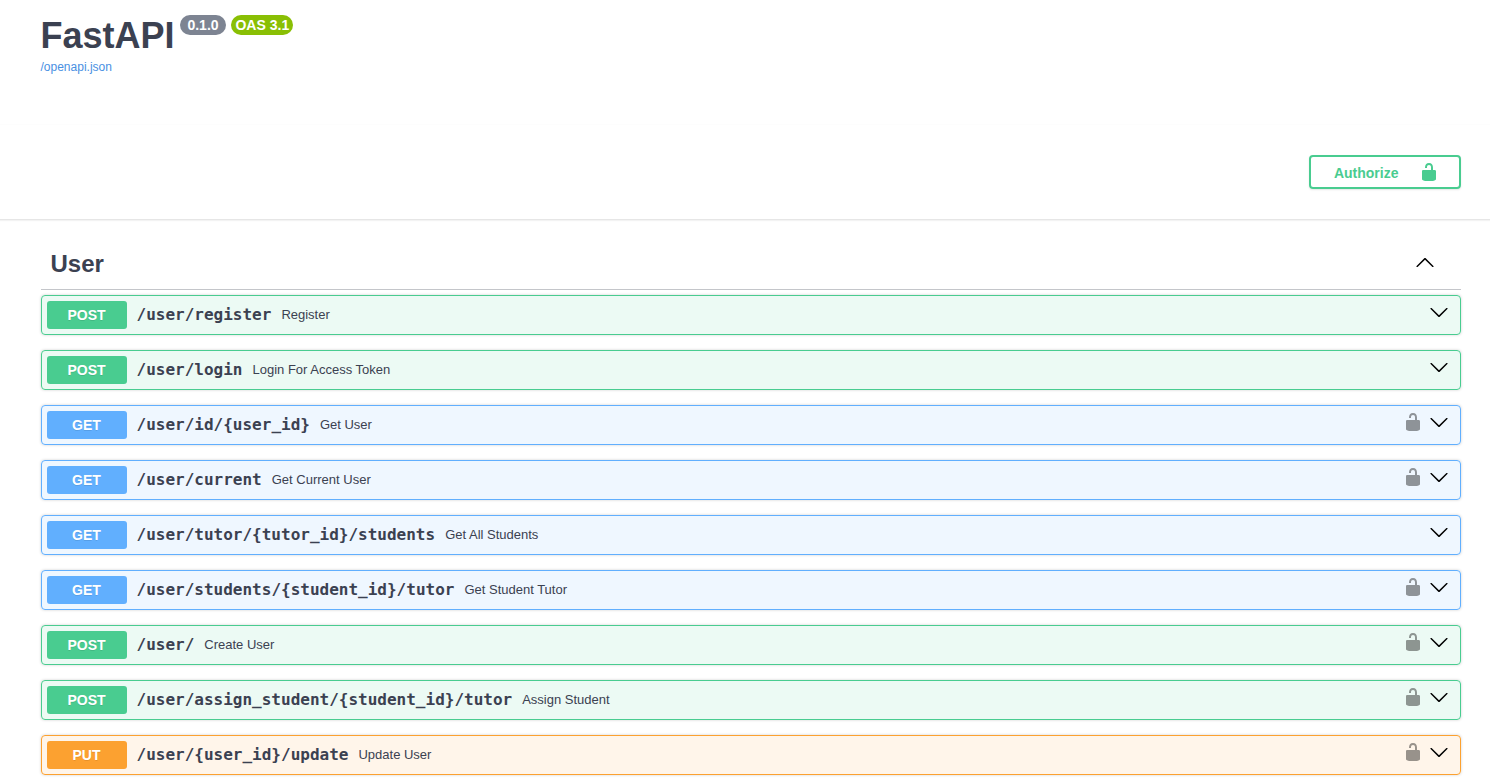
\includegraphics[width=\tamInterfaz\textwidth]{figuras/estado_arte/tecnologias/swaggerinterfaz.PNG}
        \caption{Swagger interfaz. Fuente: Elaboración propia}
        \label{fig:swaggerinterfaz}
    \end{figure}

    \item \textbf{\href{https://expressjs.com/}{Express.js} \cite{express2026home} (\ref{fig:expresslogo}):} Framework minimalista de JavaScript. Es adecuado para una amplia gama de proyectos y cuenta con una de las comunidades más grandes. No obstante, no impone una estructura, pudiendo generar problemas de mantenimiento en proyectos grandes

    \begin{figure}[ht]
        \centering
        
\includegraphics[width=\tamApps\textwidth]{figuras/estado_arte/tecnologias/expresslogo.png}
        \caption{Express Logo}
        \label{fig:expresslogo}
    \end{figure}

    \item \textbf{\href{https://nestjs.com/}{NestJS} \cite{nest2026home} (\ref{fig:nestlogo}):} Plataforma usada en JavaScript y TypeScript que aporta una estructura profesional y organizada basada en módulos y decoradores. Establece una arquitectura altamente robusta, facilitando el testing y el trabajo en equipos grandes. Como punto negativo, presenta una curva de aprendizaje elevada.

    \begin{figure}[ht]
        \centering
        
\includegraphics[width=\tamApps\textwidth * \real{1.6}]{figuras/estado_arte/tecnologias/nestlogo.png}
        \caption{Nest Logo}
        \label{fig:nestlogo}
    \end{figure}

    \item \textbf{\href{https://spring.io/projects/spring-boot}{Spring Boot} \cite{springboot2026home} (\ref{fig:springlogo}):} Framework robusto y escalable orientado a aplicaciones empresariales. Spring Boot simplifica la configuración y el despliegue de servicios web. Aporta seguridad, alta fiabilidad y mantenimiento a largo plazo.

    \begin{figure}[ht]
        \centering
        
\includegraphics[width=\tamApps\textwidth]{figuras/estado_arte/tecnologias/springlogo.png}
        \caption{Spring Logo}
        \label{fig:springlogo}
    \end{figure}

    \item \textbf{\href{https://laravel.com/}{Laravel} \cite{laravel2026home}:} Facilita el desarrollo rápido de aplicaciones webs y APIs. Contiene herramientas que conceden autenticación, validación y acceso a bases de datos. Es sencillo y eficaz para proyectos medianos. Utiliza el panel de administrador propio que podemos ver en la Figura~\ref{fig:laravelinterfaz}

    \begin{figure}[ht]
        \centering
        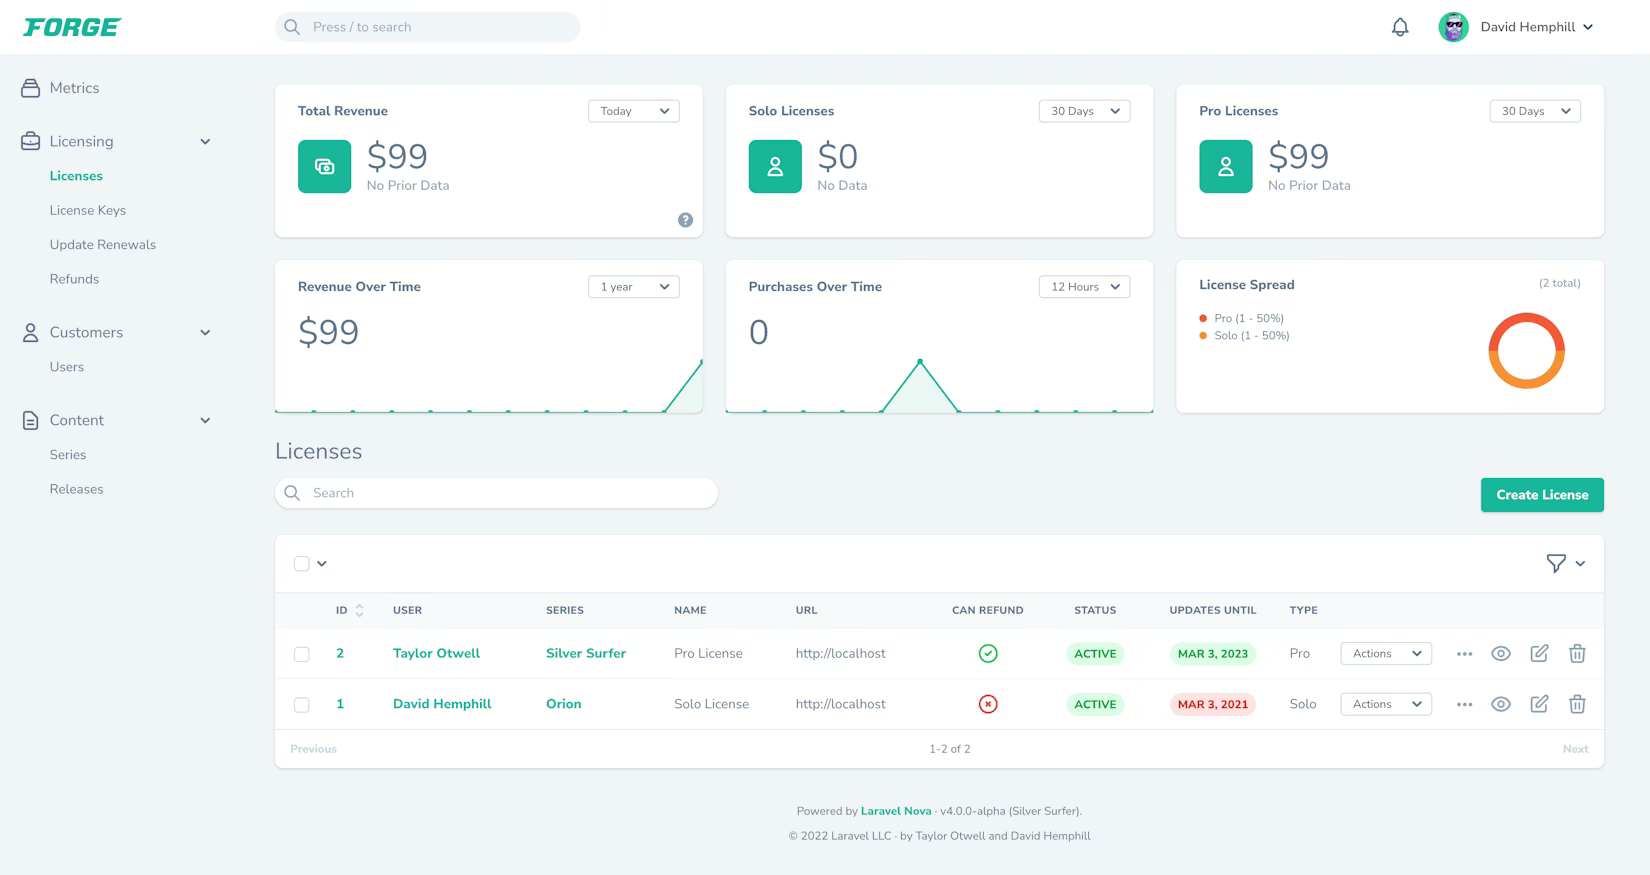
\includegraphics[width=\tamInterfaz\textwidth]{figuras/estado_arte/tecnologias/laravelinterfaz.png}
        \caption{Laravel interfaz}
        \label{fig:laravelinterfaz}
    \end{figure}

    \item \textbf{\href{https://dotnet.microsoft.com/en-us/apps/aspnet}{ASP.NET Core} \cite{aspnet2026home}:} Plataforma de alto rendimiento desarrollada por Microsoft y perteneciente al ecosistema .NET. Permite crear APIs seguras y escalables, con buena integración en entornos cloud. Se usa en proyectos empresariales y profesionales. Asimismo, hace uso de la interfaz de Swagger que podemos ver en la Figura ~\ref{fig:swaggerinterfaz}

    \item \textbf{\href{https://firebase.google.com/}{FireBase} \cite{aspnet2026home} (\ref{fig:firebaselogo}):} Plataforma de Google que ofrece servicios listos para usar como autenticación, base de datos y notificaciones. Reduce la necesidad de crear y mantener un servidor propio. Se utiliza en proyectos pequeños o con tiempo de desarrollo limitados.

    \begin{figure}[ht]
        \centering
        
\includegraphics[width=\tamApps\textwidth]{figuras/estado_arte/tecnologias/firebaselogo.png}
        \caption{Firebase Logo}
        \label{fig:firebaselogo}
    \end{figure}

    \item \textbf{\href{https://rubyonrails.org/}{Ruby on Rails} \cite{rubyonrails2026home} (\ref{fig:rubyonrailslogo}):} Framework de desarrollo web basado en Ruby. Sigue el patrón modelo-vista-controlador. Es de fácil uso y flexible. Posée sintaxis sencilla, es orientado a objetos y permite cambios de manera sencilla en el código.

    \begin{figure}[ht]
        \centering
        
\includegraphics[width=\tamApps\textwidth]{figuras/estado_arte/tecnologias/rubyonrailslogo.png}
        \caption{Ruby on Rails Logo}
        \label{fig:rubyonrailslogo}
    \end{figure}

    \item \textbf{Supabase:} Plataforma Backend-as-a-Service de código abierto basada en PostgreSQL. Aporta una API REST, servicios de autenticación, almacenamiento de archivos y control de acceso. Especialmente adecuada para aplicaciones con múltiples usuarios y necesidad de sincronización en tiempo real


\end{itemize}

\subsection{Base de Datos}

    \subsubsection{Relaciones:}

    \begin{itemize}

        \item \textbf{\href{https://www.postgresql.org/}{PostgreSQL} \cite{postgresql} (\ref{fig:postgresqllogo}):} Consta de soporte para consultas complejas y alto rendimiento. Es muy robusta y esclable, siendo ideal para manejar grandes volúmenes de datos o lógica compleja.

        \begin{figure}[ht]
        \centering
        
\includegraphics[width=\tamApps \textwidth * \real{0.6}]{figuras/estado_arte/tecnologias/postgresql.png}
        \caption{PostgreSQL Logo}
        \label{fig:postgresqllogo}
    \end{figure}
    
        \item \textbf{\href{https://www.mysql.com/}{MySQL} \cite{mysql2026home} (\ref{fig:mysqllogo}) o \href{https://mariadb.org/}{MariaDB} \cite{mariadb2026home} (\ref{fig:mariadblogo}):} Es de fácil uso. Utiliza tablas y relaciones garantizando la integridad de los datos. Es adecuado para la mayoría de aplicaciones móviles.

        \begin{figure}[ht]
        \centering
        
\includegraphics[width=\tamApps\textwidth * \real{1.8}]{figuras/estado_arte/tecnologias/mysqllogo.png}
        \caption{MySQL Logo}
        \label{fig:mysqllogo}
    \end{figure}

    \begin{figure}[ht]
        \centering
        
\includegraphics[width=\tamApps\textwidth * \real{1.8}]{figuras/estado_arte/tecnologias/mariadblogo.png}
        \caption{MariaDB Logo}
        \label{fig:mariadblogo}
    \end{figure}

        \item \textbf{\href{https://sqlite.org/}{SQLite} \cite{sqllite2026home} (\ref{fig:sqllitelogo}):} Base de datos ligera que no necesita servidor ya que se ejecuta localmente. Es usada para almacenamiento local, caché o funcionamiento sin conexión a internet.

        \begin{figure}[ht]
        \centering
        
\includegraphics[width=\tamApps\textwidth * \real{1.6}]{figuras/estado_arte/tecnologias/sqllitelogo.png}
        \caption{SQLite Logo}
        \label{fig:sqllitelogo}
    \end{figure}

    \end{itemize}


    \subsubsection{No relacionales:}

        \begin{itemize}

            \item \textbf{\href{https://www.mongodb.com/}{MongoDB} \cite{mongoDB2026home}:} Almacena la información en formato JSON. Es flexible, escalable e ideal para aplicaciones con estructuras de datos cambiantes. Para utilizarlo podemos hacer uso de la interfaz MongoDB Compass que podemos observar en la Figura~\ref{fig:mongodbinterfaz}

            \begin{figure}[ht]
        \centering
        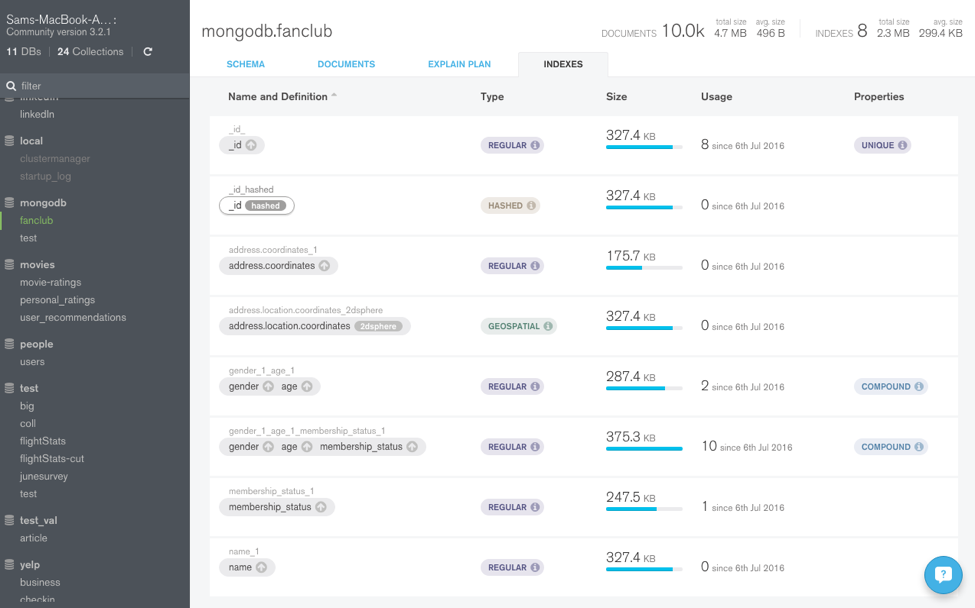
\includegraphics[width=\tamInterfaz\textwidth]{figuras/estado_arte/tecnologias/mongodb.png}
        \caption{MongoDB Compass interfaz}
        \label{fig:mongodbinterfaz}
    \end{figure}
        
            \item \textbf{\href{https://firebase.google.com/}{Firebase Firestore} \cite{firebase2026home} o \href{https://firebase.google.com/docs/database}{Realtime Database} \cite{realtime2026home} (\ref{fig:firebaselogo}):} Es almacenada en la nube y sincronizada en tiempo real. Es muy útil para aplicaciones colaborativas o con notificaciones instantáneas.

        
            \item \textbf{\href{https://redis.io/}{Redis} \cite{redis2026home} (\ref{fig:redislogo}):} Su almacenamiento es guardado en memoria y es extremadamente rápida mejorando el rendimiento. Se usa principalmente para caché, gestión de sesiones o colas de tareas. 

            \begin{figure}[ht]
        \centering
        
\includegraphics[width=\tamApps\textwidth]{figuras/estado_arte/tecnologias/redislogo.png}
        \caption{Redis Logo}
        \label{fig:redislogo}
    \end{figure}
    
        \end{itemize}
